\documentclass[a4paper,12pt]{article}

\usepackage{fancyhdr}
\usepackage{lastpage}
\usepackage{amsmath}
\usepackage{tikz}
\usepackage{amsfonts}
\usepackage{graphicx}

\newcommand{\V}[1]{\ensuremath{\vec{#1}}}
\newcommand{\F}[2]{\ensuremath{\frac{#1}{#2}}}
\newcommand{\Q}[1]{\newpage \section*{#1}}
\newcommand{\acc}[1]{\overset{..}{#1}}
\newcommand{\vel}[1]{\overset{.}{#1}}
\newcommand{\prt}[2]{\frac{\partial#1}{\partial#2}}
\newcommand{\LP}{\left(}
\newcommand{\RP}{\right)}


\pagestyle{fancy}
\lhead{Samuel Loomis}
\setlength{\headheight}{15pt}
\chead{Classical Mechanics HW 7}
\rhead{15 November 2013}
\lfoot{}
\cfoot{\thepage\ of \pageref{LastPage}}
\rfoot{}

\begin{document}

\section*{Question 1, Thornton \& Marion, 7-24}

Consider a simple plane pendulum consisting of a mass $m$ attached to a string of length $l$. After the pendulum is set into motion, the length of the string is shortened at a constant rate. \[\F{\partial{l}}{\partial{t}}=-\alpha=constant\] The suspension point remains fixed. Compute the Lagrangian and Hamiltonian functions. Compare the Hamiltonian and the total energy, and discuss the conservation of energy for the system.
\\
\begin{figure}
\centering
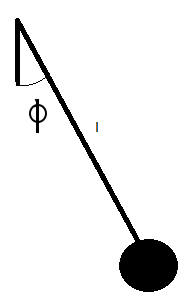
\includegraphics[width=2in]{Pendulum.png}
\end{figure}\\
The position of the pendulum at any point in time is:
\[\V{r}=lsin(\phi)\hat{x}-lcos(\phi)\hat{y}\]
The length $l$ and the angle $\phi$ are both functions of time. Taking the time derivative of $r$ gives:
\[\vel{r}=[\vel{l}sin(\phi)+lcos(\phi)\vel{\phi}]\hat{x}-[\vel{l}cos(\phi)-lsin(\phi)\vel{\phi}]\hat{y}\\\]
The velocity will be used in the kinetic energy, $v^2$:
\begin{align*}
\vel{r}^2=&\vel{l}^2sin^2(\phi)+l^2cos^2(\phi)\vel{\phi}^2+2\vel{l}l\vel{\phi}sin(\phi)cos(\phi)\\
&+\vel{l}^2cos^2{\phi}+l^2sin^2(\phi)\vel{\phi}^2-2\vel{l}l\vel{\phi}sin(\phi)cos(\phi)\\
\vel{r}^2=&\vel{l}^2+l^2\vel{\phi}^2
\end{align*}\\
The kinetic energy $T$ is:
\[T=\F{1}{2}m(\vel{l}^2+l^2\vel{\phi}^2)\]
The potential energy of this system is $mgh$, where $h$ is a time dependent function of $l$ and $\phi$:
\[h=-lcos(\phi)\]
The potential energy $U$ is:
\[U=-mglcos(\phi)\]
The Lagrangian becomes:
\[\mathcal{L}=\F{1}{2}m(\vel{l}^2+l^2\vel{\phi}^2)+mglcos(\phi )\]
The Hamiltonian is equal to:
\[\mathcal{H}=\overset{n}{\underset{i=1}{\Sigma}}p_i\vel{q}_i-\mathcal{L},where~ p_i=\F{\partial\mathcal{L}(q,\vel{q},t)}{\partial\vel{q_i}}\]
As stated earlier, both $l$ and $\phi$ equations vary with time and thus the Hamiltonian needs to be processed with respect to both equation sets.\\
$\vel{l}$:
\[p_l=\prt{\mathcal{L}}{\vel{l}}=m\vel{l}: \vel{l}=\F{p_l}{m}\]
$\vel{\phi}$:
\[p_\phi=\prt{\mathcal{L}}{\vel{\phi}}=ml^2\vel\phi:\vel\phi=\F{p_\phi}{ml^2}\]
Writing $\mathcal{H}$ in terms of $p_\phi, p_l, \phi, l$:
\begin{align*}
\mathcal{H}&=\F{p_l^2}{m}+\F{p_\phi^2}{ml^2}-\F{1}{2}m\LP\F{p_l^2}{m^2}+l^2\F{p_\phi^2}{m^2l^4}\RP-mglcos(\phi)\\
&=\F{1}{2}\left[\F{p_l^2}{m}+\F{p_\phi^2}{ml^2}\right]-mglcos(\phi)
\end{align*}
Hamiltonian's equations:
\[\vel{q}=\prt{\mathcal{H}}{p}~~~~\text{and}~~~~\vel{p}=\prt{\mathcal{H}}{q}\]
$\vel{l}$:
\[\vel{l}=\prt{\mathcal{H}}{p_l}=\F{p_l}{m}\]
$\vel{p}_l$:
\[\vel{p}_l=\prt{\mathcal{H}}{l}=-\F{p_\phi^2}{ml^3}-mgcos(\phi)\]
$\vel{\phi}$:
\[\vel{\phi}=\prt{\mathcal{H}}{p_\phi}=\F{p_\phi}{ml^2}\]
$\vel{p}_\phi$:
\[\vel{p}_\phi=\prt{\mathcal{H}}{\phi}=mglsin(\phi)\]
At this point I was informed that all I needed for this problem is $\mathcal{L}$ and $\mathcal{H}$:
\[\mathcal{L}=\F{1}{2}m(\vel{l}^2+l^2\vel{\phi}^2)+mglcos(\phi )\]
\begin{align*}
\mathcal{H}&=\F{1}{2}\left[\F{p_l^2}{m}+\F{p_\phi^2}{ml^2}\right]-mglcos(\phi)\\
&=\F{1}{2}m(\vel{l}^2+l^2\vel{\phi}^2)-mglcos(\phi )
\end{align*}
The total energy is equal to the Hamiltonian in this case.  Intuitively, the energy is not conserved due to an external force being applied to the string...  This force is supplying the system with more potential energy from the height ot the bob, but is the kinetic energy reduced at the same rate?  Anyrate, I don't think the energy is conserved due to the external force applied to the string.
Taking the derivative of the Hamiltonian with respect to time gives:
\begin{align*}
\mathcal{H}&=\F{1}{2}m(\alpha^2\vel{\phi}^2)-mglcos(\phi)\\
\prt{\mathcal{H}}{t}&=m\alpha l\vel{\phi}^2+ml^2\vel{\phi}-mg\alpha cos(\phi)+mglsin(\phi)
\end{align*}
This result shows that the Hamiltonian is changing, and thus the total energy is not conserved.
\Q{Problem 2, Thornton \& Marion, 7-31}
A spherical pendulum consists of a bob of mass $m$ attached to a weightless, extension rod of length $l$. The end of the rod opposite the bob pivots freely (in all directions) about some fixed point. Set up the Hamiltonian function in spherical coordinates.  (If $p_\phi=0$, the result is the same as that for the plane pendulum.)  Combine the term that depends on $p_\phi$ with the ordinary potential energy to find the effective potential $V(\theta,p_\phi)$.  Sketch $V$ as a function of $\theta$ for several values of $p_\phi$, including $p_\phi=0$. Discuss the features of the motion, pointing out the differences between $p_\phi=0$ and $p_\phi\ne0$. Discuss the limiting case of the conical pendulum ($\theta$=constant) with reference to the $V-\theta$ diagram.
The velocity squared used in kinetic energy can be found by taking the $dr$ vector dotted with itself and dividing it by dt squared.  The $dr$ vector in spherical is:
\[d\V{r}=dr\hat{r}+rd\theta\hat{\theta}+rsin(\theta)d\phi\hat{\phi}\]
$dr\cdot dr$ :
\[d\V{r}\cdot d\V{r}=dr^2=dr^2+r^2d\theta^2+r^2sin^2(\theta)d\phi^2\]
Dividing both sides by $dt^2$ gives:
\begin{align*}
\F{d\V{r}^2}{dt^2}&=\F{dr^2}{dt^2}+r^2\F{d\theta^2}{dt^2}+r^2sin^2(\theta)\F{d\phi^2}{dt^2}\\
\V{\vel{r}}^2&=\vel{r}^2+r^2\vel{\theta}^2+r^2sin^2(\theta)\vel{\phi}^2
\end{align*}
The kinetic energy is equal to:
\[T=\F{1}{2}m[\vel{r}^2+r^2\vel{\theta}^2+r^2sin^2(\theta)\vel{\phi}^2]\]
$r=l$ and $\vel{r}=\vel{l}=0$:
\[T=\F{1}{2}m[l^2\vel{\theta}^2+l^2sin^2(\theta)\vel{\phi}^2]\]
The potential energy is again mgh.  h in this case is equal to:
\[h=lcos(\theta)\]
\[U=mglcos(\theta)\]
The Lagrangian is equal to:
\[\mathcal{L}=\F{1}{2}m[l^2\vel{\theta}^2+l^2sin^2(\theta)\vel{\phi}^2]-mglcos(\theta)\]
The Hamiltonian:\\
$\theta$:
\[p_\theta=\prt{\mathcal{L}}{\vel{\theta}}=ml^2\vel{\theta}~~~\vel{\theta}=\F{p_\theta}{ml^2}\]
$\phi$:
\[p_\phi=\prt{\mathcal{L}}{\vel{\phi}}=ml^2sin^2(\theta)\vel{\phi}~~~\vel{\phi}=\F{p_\phi}{ml^2sin^2(\theta)}\]
The Hamiltonian is:
\[\mathcal{H}=\F{1}{2}\left[\F{p_\theta^2}{ml^2}+\F{p_\phi^2}{ml^2sin^2(\theta)}\right]+mglcos(\theta)\]
$V(\theta,p_\phi)$:
\[V(\theta,p_\phi)=\F{p_\phi^2}{2ml^2sin^2(\theta)}+mglcos(\theta)\]
Some mathematica sketches:\\
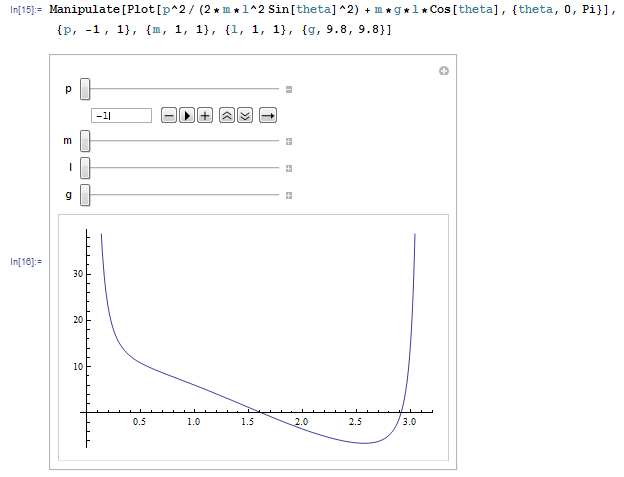
\includegraphics[width=4in]{negative_p.png}\\
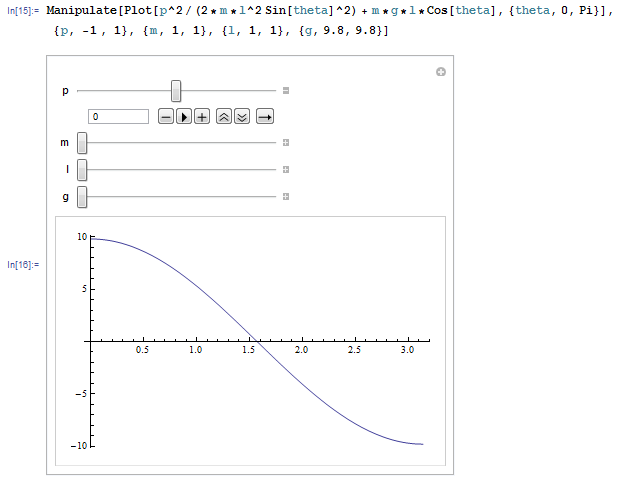
\includegraphics[width=4in]{zero_p.png}\\
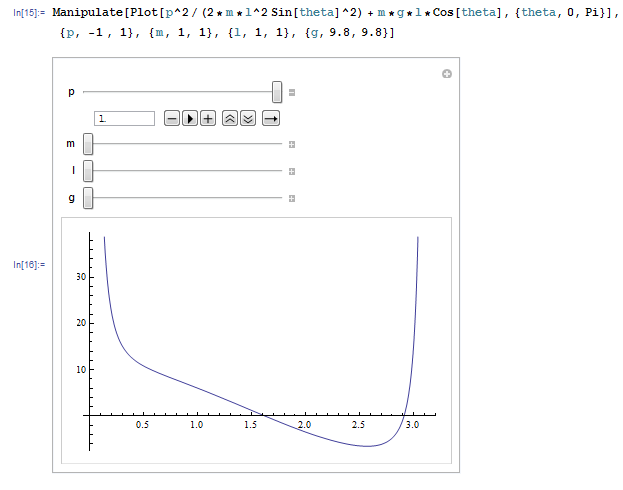
\includegraphics[width=4in]{positive_p.png}\\
When the momentum in the $\phi$ direction is 0, the potential energy is max at $\theta=0$ and the kinetic energy is max at $\theta = \pi$.  Looking at the graph for the $\phi$ momentum $\ne0$ the potential energy goes to infinity near $\theta=0$ and $\theta=\pi$, knowing that the total energy will have an upper cap and this restricts $\theta$ to be in between the values that give that maximum energy as potential.  When $\theta$ is constant, the potential energy, and thus kinetic energy doesn't change.  The pendulum will circle around at one level.  If the $\phi$ momentum is 1 as in the graph shown, and $\theta$ equals the point of the lowest potential energy, the pendulum will be in a stable circular path.

\Q{Problem 3, Taylor 13.5}
A bead of mass $m$ is threaded on a frictionless wire that is bent into a helix with cylindrical polar coordinates ($\rho$, $\phi$, $z$) satisfying $z = c\phi$ and $\rho = R$ with $c$ and $R$ constants. The $z$ axis points vertically up and gravity vertically down.  Using $\phi$ as your generalized coordinate, write down the kinetic and potential energies and the Hamiltonian $\mathcal{H}$ as a function of $\phi$ and its conjugate momentum $p$. Write down Hamilton's equations and solve for $\acc{\phi}$ and hence $\acc{z}$.  Explain your result in terms of Newtonian mechanics and discuss the special case that $R=0$.\\
The position at any point in time is equal to:
\[\V{r}=R\hat{r}+c\phi\hat{z}\]
The velocity is:
\[\vel{\V{r}}=R\vel{\phi}\hat{\phi}+c\vel{\phi}\hat{z}\]
The kinetic energy is:
\[T=\F{1}{2}m(R^2+c^2)\vel{\phi}^2\]
The potential energy is:
\[U=cmg\phi\]
The Hamiltonian is:
\[\mathcal{H}=T+U=\F{1}{2}m(R^2+c^2)\vel{\phi}^2+cmg\phi\]
The generalized momentum is:
\[p=\prt{T}{\vel{\phi}}=m(R^2+c^2)\vel{\phi}~~~\vel{\phi}=\F{p}{m(R^2+c^2)}\]
Hamiltonian rewritten:
\[\mathcal{H}=\F{p^2}{2m(R^2+c^2)}+cmg\phi\]
Hamilton's equations:
$\vel{q}$:
\[\vel{\phi}=\prt{\mathcal{H}}{p}=\F{p}{m(R^2+c^2)}\]
$\vel{p}$:
\[\vel{p}=\prt{\mathcal{H}}{\phi}=cmg\]
$\acc{\phi}$
\[\acc{\phi}=\F{d\vel{\phi}}{dt}=\F{\vel{p}}{m(R^2+c^2)}=\F{cg}{R^2+c^2}\]
$\acc{z}$:
\[\acc{z}=\F{c^2g}{R^2+c^2}=\F{g}{\F{R^2}{c^2}+1}\]
In the case that $R\rightarrow0$ the z acceleration goes to g, which makes perfect sense as the bead will be falling straight down. As R increases from this point, the acceleration in the z direction will be slower as expected, as there will be a normal force countering the force of gravity.


\end{document}